\chapter{Orígenes de Joint Embedding: Redes Siamesas y el Colapso de Representación}
\label{cap:siamesas_colapso}

La idea de comparar representaciones en lugar de reconstruir entradas físicas se remonta a principios de los 90, con la introducción de las redes siamesas. Sin embargo, este paradigma no tardó en toparse con un obstáculo fundamental: el Representation Collapse (o Colapso de Representación). En este capítulo se analizan formalmente las redes siamesas y se deducen matemáticamente las causas de este colapso.

\section{Las Redes Siamesas de Bromley (1993)}
\label{sec:siamesas_bromley}

Las redes siamesas fueron concebidas por Jane Bromley y Yann LeCun en Bell Labs \cite{bromley1993signature} para resolver el problema práctico de la verificación de firmas manuscritas. La idea central es construir un encoder que proyecte datos pertenecientes a una misma persona (misma clase semántica) a puntos cercanos en el espacio de embeddings $\mathcal{Z}$, y firmas de distintas personas (o firmas fraudulentas) a puntos distantes.

\begin{definition}[Arquitectura de Red Siamesa]
Sea $\mathcal{X} \subseteq \mathbb{R}^D$ el espacio de imágenes de entrada. Consideremos un único modelo de red neuronal parametrizado por un vector de pesos $W \in \mathbb{R}^M$, que define una función diferenciable $f_W: \mathbb{R}^D \to \mathbb{R}^d$. 
La arquitectura siamesa consta de dos copias idénticas de esta función (que comparten exactamente el mismo vector de parámetros $W$). Dadas dos entradas $x_1, x_2 \in \mathcal{X}$, la red calcula sus embeddings en paralelo:
\begin{equation}
z_1 = f_W(x_1), \quad z_2 = f_W(x_2)
\end{equation}

La métrica de distancia en el espacio latente se define mediante la distancia euclídea:
\begin{equation}
d_W(x_1, x_2) = \| f_W(x_1) - f_W(x_2) \|_2
\end{equation}
\end{definition}

Aunque la distancia euclídea $d_W$ mide la disimilitud geométrica, en la formulación de la pérdida suele emplearse su cuadrado, conocido como error cuadrático medio, para garantizar la diferenciabilidad del gradiente (distancia cuadrática, Sección~\ref{sec:loss_functions} del Apéndice~\ref{ap:fundamentos_dl}). Esta estructura de pesos compartidos garantiza que dos entradas idénticas $x_1 = x_2$ se proyecten obligatoriamente en el mismo punto del espacio $\mathcal{Z}$ $z_1 = z_2$, preservando la reflexividad de la distancia.

\section{Representation Collapse}
\label{sec:demostracion_colapso}

El colapso de representación ocurre cuando la red encuentra una solución trivial que minimiza la distancia $d_W$ entre muestras similares sin extraer características útiles de los datos.

\begin{remark}[Notación Poblacional]
\label{subsec:enfoque_probabilistico}
Esta sección se constituye desde un enfoque teórico, por tanto, a menudo se sustituirán los estimadores empíricos sobre \textit{minibatches} por sus versiones poblacionales; por ejemplo, el promedio se sustituirá por la esperanza matemática ($\mathbb{E}$) sobre la verdadera distribución de los datos ($p_{\text{pos}}$ y $p_{\text{data}}$). Aunque el entrenamiento en la práctica se realiza sobre conjuntos finitos, este enfoque permite analizar con mayor rigor las causas del colapso, eliminando el ruido y las limitaciones del muestreo empírico.
\end{remark}

\subsection{El Colapso Constante como Mínimo Global}
\label{subsec:colapso_constante}



Consideremos un escenario de entrenamiento donde únicamente disponemos de un conjunto empírico de pares compatibles (también llamados pares positivos) $\mathcal{D} = \{(x_1^{(i)}, x_2^{(i)})\}_{i=1}^N$. Estos pares representan casos compatibles, por ejemplo varias vistas de un mismo objeto o, en el caso de las redes siamesas originales, dos firmas de la misma persona. En la práctica, el objetivo de la red es minimizar el promedio de las distancias cuadráticas sobre este conjunto o sobre minibatches (Apéndice~\ref{subsec:minibatch}):

\begin{equation}
\hat{\mathcal{L}}_{\text{pos}}(W) = \frac{1}{N} \sum_{i=1}^N \| f_W(x_1^{(i)}) - f_W(x_2^{(i)}) \|_2^2
\label{eq:L_pos_empirica}
\end{equation}

Sin embargo, asumiendo que los pares provienen de una distribución conjunta $p_{\text{pos}}(x_1, x_2)$ sobre $\mathcal{X} \times \mathcal{X}$, el verdadero propósito es optimizar el modelo sobre toda la población de datos subyacente. Por ello, el análisis teórico requiere abstraerse del sumatorio empírico y definir la función de pérdida global como la esperanza matemática de la distancia cuadrática:

\begin{equation}
\mathcal{L}_{\text{pos}}(W) = \mathbb{E}_{(x_1, x_2) \sim p_{\text{pos}}} \left[ \| f_W(x_1) - f_W(x_2) \|_2^2 \right]
\label{eq:L_pos}
\end{equation}

Esta formulación basada en la esperanza y no en el estimador empírico es el estándar adoptado en la literatura \cite{wang2020understanding}. A partir de este objetivo poblacional, podemos demostrar que el colapso a constante es un mínimo global y un atractor estable del gradiente para esta función de pérdida.

\begin{figure}[H]
\centering
\begin{tikzpicture}[node distance=1.5cm, auto, >=Stealth]
    % Entradas con las imágenes de las firmas
    \node (x1) [draw, rectangle, minimum width=2.5cm, minimum height=1.5cm] {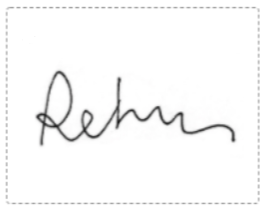
\includegraphics[width=2.3cm, height=1.3cm]{signature_Rodlf1.png}};
    \node (x2) [draw, rectangle, minimum width=2.5cm, minimum height=1.5cm, below=of x1, yshift=-0.5cm] {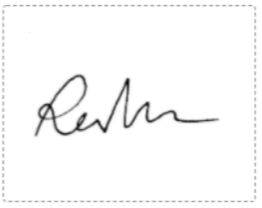
\includegraphics[width=2.3cm, height=1.3cm]{signature_Rodlf2.png}};
    
    % Textos descriptivos de las entradas
    \node [above=0.05cm of x1, font=\footnotesize] {Entrada $x_1$ (Firma A)};
    \node [below=0.05cm of x2, font=\footnotesize] {Entrada $x_2$ (Firma B)};
    
    % Encoders siameses (comparten W)
    \node (f1) [draw, rectangle, minimum width=2cm, minimum height=1cm, right=of x1, xshift=1cm] {Encoder $f_{W}$};
    \node (f2) [draw, rectangle, minimum width=2cm, minimum height=1cm, right=of x2, xshift=1cm] {Encoder $f_{W}$};
    
    % Espacio latente colapsado (z1 = z2 = c)
    \node (z) [circle, draw, double, red, thick, minimum size=1.5cm] at ($(f1.east)!0.5!(f2.east) + (2.5cm,0)$) {$z_1 = z_2 = c$};
    \node [above=0.1cm of z, font=\footnotesize\bfseries, align=center, red] {Espacio Latente $\mathcal{Z}$\\};
    
    % Pérdida (Loss)
    \node (loss) [draw, diamond, minimum width=1.5cm, minimum height=1.5cm, right=of z, xshift=0cm] {Loss = 0}; 

    % Conexiones
    \draw[->] (x1) -- (f1);
    \draw[->] (x2) -- (f2);
    \draw[->] (f1.east) -- (z.north west);
    \draw[->] (f2.east) -- (z.south west);
    \draw[->] (z) -- (loss);
    \draw[dashed, <->] (f1) -- node[left] {Shared $W$} (f2);
\end{tikzpicture}
\caption{Ilustración del colapso de representación constante en una arquitectura siamesa con firmas manuscritas. Dos entradas diferentes $x_1$ y $x_2$ correspondientes a firmas de la misma persona se proyectan por encoders idénticos $f_W$ a un único punto constante $c$ en el espacio latente $\mathcal{Z}$. Aunque este mapeo trivial minimiza la distancia $d_W(x_1, x_2)$ resultando una pérdida de cero, la representación resultante carece de valor al eliminar toda variación semántica.}
\label{fig:colapso_siamesas}
\end{figure}

\begin{theorem}[Colapso de Representación Constante]
Cualquier mapeo constante de la forma $f_{W^*}(x) = c$ para todo $x \in \mathcal{X}$, donde $c \in \mathbb{R}^d$ es un vector constante arbitrario, es un mínimo global absoluto de la función de pérdida $\mathcal{L}_{\text{pos}}(W)$.
\end{theorem}

\begin{proof}
Dado que la norma euclídea al cuadrado es no negativa por definición, tenemos que:
\begin{equation}
\| f_W(x_1) - f_W(x_2) \|_2^2 \ge 0 \quad \forall x_1, x_2 \in \mathcal{X}
\end{equation}
Tomando la esperanza matemática en ambos lados de la desigualdad, se deduce directamente que la función de pérdida está acotada inferiormente por cero:
\begin{equation}
\mathcal{L}_{\text{pos}}(W) \ge 0 \quad \forall W \in \mathbb{R}^M
\end{equation}
Evaluamos ahora la función de pérdida para el mapeo constante $f_{W^*}(x) = c$:
\begin{equation}
\mathcal{L}_{\text{pos}}(W^*) = \mathbb{E}_{(x_1, x_2) \sim p_{\text{pos}}} \left[ \| c - c \|_2^2 \right] = \mathbb{E}_{(x_1, x_2)} [ 0 ] = 0
\end{equation}
Dado que la pérdida alcanza su cota inferior global absoluta en $W^*$, el mapeo constante $f_{W^*}(x) = c$ es un mínimo global de $\mathcal{L}_{\text{pos}}(W)$.
\end{proof}


El teorema establece la existencia del colapso como mínimo global, pero no dice nada 
sobre si el descenso de gradiente converge efectivamente hacia él. Analicemos la dinámica de optimización mediante descenso de gradiente. 

Sea $\theta_k \in W$ un parámetro individual de la red. Aplicando la regla de la cadena bajo la integral (regla de Leibniz), la derivada parcial de la pérdida respecto a $\theta_k$ es:

\begin{equation}
\frac{\partial \mathcal{L}_{\text{pos}}(W)}{\partial \theta_k} = \mathbb{E}_{(x_1, x_2) \sim p_{\text{pos}}} \left[ 2 \left( f_W(x_1) - f_W(x_2) \right)^T \left( \frac{\partial f_W(x_1)}{\partial \theta_k} - \frac{\partial f_W(x_2)}{\partial \theta_k} \right) \right]
\end{equation}

En el estado colapsado $f_{W^*}(x) = c$, el factor de diferencia se anula para cualquier par:
\begin{equation}
f_{W^*}(x_1) - f_{W^*}(x_2) = c - c = \vec{0} \quad \forall\, x_1, x_2 \in \mathcal{X}
\end{equation}

Sustituyendo en la expresión del gradiente:
\begin{equation}
\frac{\partial \mathcal{L}_{\text{pos}}(W^*)}{\partial \theta_k} = \mathbb{E}_{(x_1, x_2) \sim p_{\text{pos}}} \left[ 2 \cdot \vec{0}^{\,T} \left( \frac{\partial f_W(x_1)}{\partial \theta_k} - \frac{\partial f_W(x_2)}{\partial \theta_k} \right) \right] = 0
\end{equation}

El gradiente se anula idénticamente para todo $\theta_k$, de modo que las iteraciones del descenso quedan detenidas: $W^{(t+1)} = W^{(t)} - \eta \nabla_W \mathcal{L}_{\text{pos}}(W^{(t)}) = W^{(t)}$. El estado colapsado es, por tanto, un punto fijo del optimizador.

Que sea además un \emph{atractor} se sigue de la estructura de la pérdida $\mathcal{L}_{\text{pos}}$, que únicamente penaliza la distancia entre representaciones de pares positivos, sin disponer de fuerzas contrapuesta que obligue a dispersar los embeddings. Cada paso de optimización reduce progresivamente esa distancia, contrayendo las representaciones hacia un mismo punto. 

Esta dinámica se acentúa cuando la red se inicializa cerca del colapso (p.e. con pesos pequeños) que producen embeddings casi idénticos. En ese régimen, $f_W(x_1) - f_W(x_2) \approx \vec{0}$ hace que el gradiente sea ya casi nulo, eliminando cualquier señal que pudiera diversificar las representaciones. La única dirección de actualización disponible sigue siendo contractiva, 
de modo que el optimizador no dispone de señal para escapar hacia 
representaciones más diversas. En ausencia de mecanismos que penalicen 
la contracción, esta dinámica favorece la convergencia hacia el colapso total, 
aunque el resultado depende en general de la inicialización y de la 
estructura de los datos.


\section{Colapso Dimensional}
\label{sec:colapso_dimensional_v2}

Se distinguen dos formas de degeneración geométrica en el espacio de representación. El colapso total o trivial es aquel donde el encoder contrae toda la variedad de entrada a un único punto invariante. Por el contrario, el \emph{colapso dimensional} es una patología más sutil: las representaciones escapan del punto trivial pero quedan confinadas en un subespacio propio de menor dimensión, perdiendo capacidad expresiva de forma irreversible.

\begin{definition}[Colapso Dimensional]
Sea $\mathcal{X}$ el espacio de entrada y $f_W: \mathcal{X} \to \mathbb{R}^d$ un encoder parametrizado por los pesos $W$, donde $d$ representa la dimensionalidad de salida. Aunque la pérdida de la red se optimiza midiendo distancias sobre pares compatibles ($p_{\text{pos}}$), la riqueza o expresividad del espacio latente se evalúa comprobando la diversidad de todas las imágenes de forma global. Por ello, definimos formalmente la matriz de covarianza del espacio de representaciones evaluando la esperanza sobre la distribución $p_{\text{data}}$ (Apéndice~\ref{sec:al_covarianza_rango}):
\begin{equation}
    \Sigma_\mathcal{Z} = \mathbb{E}_{x \sim p_{\text{data}}}\left[(f_W(x) - \mu)(f_W(x) - \mu)^T\right] \in \mathbb{R}^{d \times d}
\end{equation}
donde $\mu = \mathbb{E}_{x \sim p_{\text{data}}}[f_W(x)] \in \mathbb{R}^d$ es el vector de medias del espacio $\mathcal{Z}$. Decimos que la representación sufre colapso dimensional si:
\begin{equation}
    \operatorname{rango}(\Sigma_\mathcal{Z}) = r < d.
\end{equation}
\end{definition}

\begin{remark}[Suficiencia muestral y rango empírico]
En el escenario empírico sobre un batch de tamaño $B$, se usa el estimador $\hat{\Sigma}_\mathcal{Z} = \frac{1}{B-1}(Z - \bar{Z})^T(Z - \bar{Z})$, donde $Z \in \mathbb{R}^{B \times d}$. Recordemos que si $B \le d$, la matriz es singular. El colapso dimensional es una propiedad asintótica o poblacional donde incluso si $B \gg d$, $\operatorname{rango}(\Sigma_\mathcal{Z}) = r < d$.
\end{remark}

 Usaremos el Teorema Espectral para Matrices Simétricas (Apéndice~\ref{sec:al_teorema_espectral}). Dado que $\Sigma_\mathcal{Z}$ es simétrica y semidefinida positiva, existe una base ortonormal de $\mathbb{R}^d$ formada por autovectores de $\Sigma_\mathcal{Z}$. Podemos descomponerla diagonalmente como:
\begin{equation}
    \Sigma_\mathcal{Z} = Q \Lambda Q^T = 
    \begin{pmatrix}
        | & & | \\
        q_1 & \dots & q_d \\
        | & & |
    \end{pmatrix}
    \begin{pmatrix}
        \sigma_1^2 & & & 0 \\
        & \ddots & & \\
        & & \sigma_r^2 & \\
        0 & & & \mathbf{0}_{d-r}
    \end{pmatrix}
    \begin{pmatrix}
        - & q_1^T & - \\
          & \vdots &   \\
        - & q_d^T & -
    \end{pmatrix}
\end{equation}
donde $\sigma_1^2 \ge \dots \ge \sigma_r^2 > 0$ representan la varianza de los datos a lo largo de las direcciones principales $q_i$. Por el \textbf{Teorema de la Dimensión} (Apéndice~\ref{ap:algebra_lineal}):
\begin{equation}
    \dim(\operatorname{Ker}(\Sigma_\mathcal{Z})) = d - \operatorname{rango}(\Sigma_\mathcal{Z}) = d - r.
\end{equation}
Cualquier vector $v \in \operatorname{Ker}(\Sigma_\mathcal{Z}) \subseteq \mathbb{R}^d$ constituye una dirección de colapso donde la varianza es nula. Esto significa que el encoder concentra las representaciones de los datos sobre el subespacio afín $f_W(x) \in \mu + (\operatorname{Ker}(\Sigma_\mathcal{Z}))^\perp$ para casi todo $x \sim p_{\text{data}}.$ En términos geométricos, al carecer de varianza, a lo largo de las direcciones del núcleo los datos no se desvían de su media $\mu$ colapsando esas dimensiones a constante.

\begin{proposition}[Estabilidad del Colapso Dimensional]
Sea $f_W$ un encoder parametrizado por $W$ y sea $W^*$ un estado de la red donde $\operatorname{rango}(\Sigma_\mathcal{Z}) = r < d$. Para todo vector del núcleo $v \in \operatorname{Ker}(\Sigma_\mathcal{Z}) \subseteq \mathbb{R}^d$, la varianza de las proyecciones sobre $v$ es nula, es decir, $v^T f_{W^*}(x)$ es constante para casi todo $x \sim p_{\text{data}}.$ 

Dado que las distribuciones marginales de los pares en $p_{\text{pos}}$ coinciden exactamente con $p_{\text{data}}$ (cada elemento del par es una muestra de la distribución real), se cumple que $v^T(f_{W^*}(x) - f_{W^*}(x^+)) = 0$ para casi todo $(x, x^+) \sim p_{\text{pos}}$, y por la regla de la cadena, la componente de cualquier gradiente derivado de la pérdida positiva $\mathcal{L}_{\text{pos}}$ que intente actualizar las representaciones en la dirección $v$ es idénticamente nula. Por tanto, el subespacio nulo es un invariante algebraico bajo la dinámica de optimización:
\begin{equation}
    v^T \nabla_{f_W} \mathcal{L}_{\text{pos}}(W^*) = 0.
\end{equation}
\end{proposition}

\subsection*{Mecanismo Dinámico: El Flujo de Gradiente como Operador de Contracción}

La proposición anterior ilustra de manera general por qué el colapso es un estado absorbente, pero no explica el proceso dinámico mediante el cual el sistema precipita hacia él. Siguiendo el marco analítico establecido por Jing et al.~\cite{jing2022understanding} para el estudio del flujo de gradiente en redes siamesas, descompondremos el factor lineal de la capa final $f_W(x) = W\phi(x)$ (Apéndice~\ref{subsec:capa_proyeccion}), con pesos $W \in \mathbb{R}^{d \times m}$ y siendo $\phi(x) \in \mathbb{R}^{m}$ la salida de la capa $L-1$ (siendo $L$ el número de capas).

\begin{figure}[H]
\centering
\begin{tikzpicture}[node distance=0.8cm, auto, >=Stealth]
    % Nodos de la arquitectura
    \node (x) [draw, rectangle, rounded corners, minimum width=1.2cm, minimum height=1cm, fill=gray!10, font=\footnotesize] {Entrada $x$};
    
    \node (encoder) [draw, rectangle, minimum width=2.4cm, minimum height=1.2cm, right=of x, fill=blue!5, align=center, font=\footnotesize] {Encoder no lineal\\(Capas $1$ a $L-1$)};
    
    \node (phi) [draw, circle, inner sep=1pt, minimum size=0.9cm, right=of encoder, fill=green!5, font=\footnotesize] {$\phi(x)$};
    \node [above=0.1cm of phi, font=\scriptsize, align=center] {Pre-activ.\\$\mathbb{R}^m$};
    
    \node (W) [draw, rectangle, minimum width=1.8cm, minimum height=1.2cm, right=of phi, fill=orange!5, align=center, font=\footnotesize] {Proyección\\Lineal $W$};
    
    \node (f) [draw, circle, double, inner sep=1pt, minimum size=0.9cm, right=of W, fill=red!5, font=\footnotesize] {$f_W(x)$};
    \node [above=0.1cm of f, font=\scriptsize, align=center] {Espacio lat.\\$\mathbb{R}^d$};

    % Flechas de flujo de datos
    \draw[->, thick] (x) -- (encoder);
    \draw[->, thick] (encoder) -- (phi);
    \draw[->, thick] (phi) -- (W);
    \draw[->, thick] (W) -- (f);
    
    % Caja general agrupando todo
    \draw[dashed, gray] ($(encoder.north west)+(-0.2,0.8)$) rectangle ($(W.south east)+(0.2,-0.4)$);
    \node[gray, font=\footnotesize] at ($(encoder.north)!0.5!(W.north) + (0, 1.1)$) {Red Neuronal Completa $f_W$};
\end{tikzpicture}
\caption{Descomposición estructural de la red neuronal para el análisis del colapso. El procesamiento de la entrada $x$ se divide en un extractor de características complejo (que engloba todas las transformaciones no lineales hasta la capa $L-1$) generando el vector $\phi(x)$, seguido de un operador puramente lineal parametrizado por la matriz $W$ que proyecta estas representaciones al espacio final.}
\label{fig:descomposicion_lineal}
\end{figure}
El objetivo de este análisis es mostrar formalmente que la pérdida $\mathcal{L}_{\text{pos}}$ actúa como un \textbf{operador contractivo} que empuja la red hacia el colapso dimensional. Para evidenciar matemáticamente esta fuerza de contracción, es indispensable separar la contribución de los parámetros $W$, de la estructura geométrica intrínseca de los datos.

Para ello, recordemos la forma general de la pérdida que queda como:
\begin{equation}
    \mathcal{L}_{\text{pos}}(W) = \mathbb{E}_{p_{\text{pos}}} \left[ \| W\phi(x) - W\phi(x^+) \|_2^2 \right].
\end{equation}

A partir de aquí, podemos reescribir la función de pérdida de forma cuadrática añadiendo el factor $\frac{1}{2}$, habitual en optimización para cancelar el exponente al derivar. Sea $\Delta \phi = \phi(x) - \phi(x^+)$ por tanto:

\begin{equation}
    \mathcal{L}_{\text{pos}}(W) = \frac{1}{2}\mathbb{E}_{p_{\text{pos}}} \left[\|W \Delta \phi\|_2^2 \right].
\end{equation}

Aplicando las propiedades: $v^T v = \|v\|_2^2 $, $v^T v = \operatorname{Tr}(v v^T)$ y $\operatorname{Tr}(AB) = \operatorname{Tr}(BA)$:

\begin{equation}
    \|W \Delta \phi\|_2^2 = \operatorname{Tr}\left( (W \Delta \phi) (W \Delta \phi)^T \right) = \operatorname{Tr}\left( W (\Delta \phi \Delta \phi^T) W^T \right).
\end{equation}

Sustituyendo lo anterior y aplicando linealidad de la esperanza:
\begin{equation}
    \mathcal{L}_{\text{pos}}(W) = \frac{1}{2} \mathbb{E}_{p_{\text{pos}}}\left[ \| W \Delta \phi \|_2^2 \right] = \frac{1}{2} \operatorname{Tr}\left( W \mathbb{E}_{p_{\text{pos}}}\left[ \Delta \phi \Delta \phi^T \right] W^T \right).
\end{equation}

Definimos ahora la matriz de covarianza diferencial en la capa $L-1$ como:
\begin{equation}
    \Sigma_{\Delta} = \mathbb{E}_{p_{\text{pos}}}\left[(\phi(x) - \phi(x^+))(\phi(x) - \phi(x^+))^T\right] \in \mathbb{R}^{m \times m}.
\end{equation}

Sustituyendo esta definición, la pérdida se expresa como forma cuadrática: 

\begin{equation}
    \mathcal{L}_{\text{pos}}(W) = \frac{1}{2} \operatorname{Tr}\left( W \Sigma_{\Delta} W^T \right).
\end{equation}
\vspace{10pt}

Para estudiar la dinámica del descenso de gradiente resulta conveniente considerar el sistema dinámico continuo asociado, conocido como Gradient Flow (Apéndice~\ref{sec:al_flujo_gradiente}):

\begin{equation}
    \dot{W}(t) = -\nabla_W \mathcal{L}_{\text{pos}}(W(t)).
\end{equation}

Como $\mathcal{L}_{\text{pos}}$ es una forma cuadrática, $-\nabla_W \mathcal{L}_{\text{pos}}(W(t))= -W(t) \Sigma_{\Delta}$ y por tanto:

\begin{equation}
    \dot{W}(t) = -W(t) \Sigma_{\Delta}.
\end{equation}

A continuación, resolvemos el sistema para estudiar su convergencia. Siguiendo a Jing et al.~\cite{jing2022understanding}, asumimos que la matriz de covarianza diferencial $\Sigma_{\Delta}$ es constante en el tiempo, lo que permite obtener una solución analítica cerrada.

Dado que $\Sigma_{\Delta}$ está definida como la esperanza de un producto, es por construcción una matriz \textbf{semi-definida positiva}. Aplicando el Teorema Espectral, descomponemos la matriz $\Sigma_{\Delta} = U \Lambda_{\Delta} U^T$, donde $U \in \mathbb{R}^{m \times m}$ es una matriz ortogonal ($U^T U = I$) y $\Lambda_{\Delta} = \operatorname{diag}(\lambda_1, \dots, \lambda_m)$ contiene sus autovalores. Debido a que la matriz es semi-definida positiva, se garantiza matemáticamente que todos sus autovalores son no negativos ($\lambda_j \ge 0$), representando la magnitud de la varianza de los cambios a lo largo de cada dirección geométrica principal. Introducimos el cambio de variables

\begin{equation}
    \tilde{W}(t) = W(t)U.
\end{equation}

Multiplicando la ecuación diferencial por la derecha por $U$ y utilizando que
$\Sigma_{\Delta}U = U\Lambda_{\Delta}$, obtenemos:

\begin{equation}
    \dot{W}(t)U
    = -W(t)\Sigma_{\Delta}U
    = -W(t)U\Lambda_{\Delta}.
\end{equation}

Por definición de $\tilde{W}(t)$, esto equivale a:

\begin{equation}
    \dot{\tilde{W}}(t)
    = -\tilde{W}(t)\Lambda_{\Delta}.
\end{equation}

De forma matricial:
\begin{equation}
    \begin{pmatrix}
        \dot{\tilde{w}}_{11}(t) & \dots & \dot{\tilde{w}}_{1m}(t) \\
        \vdots & \ddots & \vdots \\
        \dot{\tilde{w}}_{d1}(t) & \dots & \dot{\tilde{w}}_{dm}(t)
    \end{pmatrix} = -
    \begin{pmatrix}
        \tilde{w}_{11}(t) & \dots & \tilde{w}_{1m}(t) \\
        \vdots & \ddots & \vdots \\
        \tilde{w}_{d1}(t) & \dots & \tilde{w}_{dm}(t)
    \end{pmatrix}
    \begin{pmatrix}
        \lambda_1 & & 0 \\
        & \ddots & \\
        0 & & \lambda_m
    \end{pmatrix}
\end{equation}

Resolviendo el sistema cada componente se expresa como:
\begin{equation}
    \tilde{w}_{ij}(t) = \tilde{w}_{ij}(0) e^{-\lambda_j t}.
\end{equation}

Dado que $\lambda_j \ge 0$ podemos concluir que $\mathcal{L}_{\text{pos}}$ actúa como un operador de contracción. Sin embargo, la velocidad de esta contracción depende críticamente de la varianza de las aumentaciones. Observando el término de decaimiento $e^{-\lambda_j t}$, es evidente que aquellas direcciones $j$ asociadas a autovalores \textbf{grandes} ($\lambda_j \gg 0$) ---es decir, características pre-activación que varían fuertemente entre la imagen y su versión aumentada--- sufren una rápida contracción exponencial hacia el origen. Por el contrario, las características asociadas a autovalores pequeños ($\lambda_j \approx 0$), que son naturalmente invariantes a las aumentaciones, apenas experimentan contracción.

A menos que el framework de aprendizaje autosupervisado introduzca un mecanismo de fuerza repulsiva, la red tenderá a suprimir agresivamente cualquier dirección latente que no sea estrictamente invariante. En el momento en que las componentes no invariantes se extinguen por completo ($t \to \infty$), si el número de características supervivientes es menor que la dimensionalidad $d$, el rango de la covarianza de salida $\Sigma_\mathcal{Z}$ decae. La representación queda atrapada de manera irreversible en el subespacio degenerado protegido por la Proposición 3.1.

\begin{figure}[!ht]
%\centering
\resizebox{\linewidth}{!}{%
\begin{tikzpicture}[
    node distance=0.5cm,
    problem/.style={draw=red!70!black, rounded corners, minimum width=2cm, minimum height=1.2cm, align=center, fill=red!8, font=\scriptsize, text=black},
    solution/.style={draw=blue!70!black, rounded corners, minimum width=2cm, minimum height=1.2cm, align=center, fill=blue!8, font=\scriptsize, text=black},
    assumption/.style={draw=yellow!70!black, rounded corners, minimum width=2cm, minimum height=1.2cm, align=center, fill=yellow!10, font=\scriptsize, text=black},
    final/.style={draw=green!60!black, rounded corners, minimum width=2cm, minimum height=1.2cm, align=center, fill=green!10, font=\scriptsize, thick, text=black},
    arrow/.style={->, >=stealth, thick, gray!70},
    label/.style={font=\tiny, text=black, align=center}
]

% Nodos
\node[problem] (collapse) {Colapso\\Trivial y\\Dimensional};
\node[label, above=0.1cm of collapse] {Cap.~3\\(1993)};

\node[solution, right=of collapse] (contrastive) {P\'{e}rdidas\\Contrastivas\\$\mathcal{L}_{\text{neg}}$};
\node[label, above=0.1cm of contrastive] {Cap.~4\\(2006)};

\node[problem, right=of contrastive] (exp) {Escala\\exponencial\\$\mathcal{O}(e^d)$};

\node[solution, right=of exp] (barlow) {Barlow Twins\\VICReg\\(decorrelaci\'{o}n)};
\node[label, above=0.1cm of barlow] {Cap.~5\\(2021--2022)};

\node[assumption, right=of barlow] (gauss) {Hip\'{o}tesis\\Gaussiana\\no verificada};

\node[solution, right=of gauss] (jepa) {V-JEPA\\(heur\'{i}sticas\\ad-hoc)};
\node[label, above=0.1cm of jepa] {Cap.~6\\(2022--2025)};

\node[final, right=of jepa] (sigreg) {\textbf{SIGReg}\\Normalidad\\forzada};
\node[label, above=0.1cm of sigreg] {Cap.~7\\(2025--2026)};

% Flechas
\draw[arrow] (collapse) -- (contrastive);
\draw[arrow] (contrastive) -- (exp);
\draw[arrow] (exp) -- (barlow);
\draw[arrow] (barlow) -- (gauss);
\draw[arrow] (gauss) -- (jepa);
\draw[arrow] (jepa) -- (sigreg);

% Arco de cierre
\draw[->, >=stealth, thick, green!50!black, dashed] (sigreg.south) to[out=-90, in=-90, looseness=0.5] node[below, font=\scriptsize\itshape, text=green!50!black, yshift=-0.1cm] {Cierre del Principio de Barlow} (barlow.south);

% Leyenda
\node[below=1.8cm of collapse, font=\scriptsize, anchor=west] (leg) {
    {\tikz\draw[fill=red!8, draw=red!70!black, rounded corners] (0,0) rectangle (0.4,0.25);} Problema \quad
    {\tikz\draw[fill=blue!8, draw=blue!70!black, rounded corners] (0,0) rectangle (0.4,0.25);} Soluci\'{o}n \quad
    {\tikz\draw[fill=yellow!10, draw=yellow!70!black, rounded corners] (0,0) rectangle (0.4,0.25);} Hip\'{o}tesis pendiente \quad
    {\tikz\draw[fill=green!10, draw=green!60!black, rounded corners] (0,0) rectangle (0.4,0.25);} Resoluci\'{o}n final
};

\end{tikzpicture}%
}
\caption[Flujo conceptual del trabajo y hoja de ruta.]{El colapso de representación descrito en este capítulo (rojo) motivó la búsqueda de fuerzas repulsivas. En los siguientes capítulos se estructuran propuestas posteriores y sus limitaciones}
\label{fig:roadmap_cap3}

\vspace{7pt}
Este capítulo ha demostrado que la pérdida $\mathcal{L}_{\text{pos}}$, por sí sola, conduce inevitablemente al colapso del espacio de representaciones, tanto en su forma trivial (constante) como en su forma dimensional (reducción de rango). A continuación se ilustra el flujo de ideas que se irá desarrollando a lo largo de los capítulos siguientes para resolver este problema central en las \emph{JEA}

En los siguientes capítulos analizaremos diferentes  mecanismos para incluir estas fuerzas repulsivas, vía términos contrastivos como $\mathcal{L}_{\text{neg}}$, o mediante restricciones explícitas sobre la geometría del espacio latente como las penalizaciones de decorrelación en VICReg o Barlow Twins.
Cada limitación identificada motiva la solución posterior, formando un camino evolutivo que aún sigue abierto~\cite{klindt2026lejepa}.
\begin{itemize}
    \item \textbf{Capítulo 3 (1993--2006)}: se formaliza el problema del colapso trivial (donde la red mapea todas las muestras a una constante) y el colapso dimensional (reducción de rango del espacio latente).
    \item \textbf{Capítulo 4 (2006--2020)}: se introduce el aprendizaje contrastivo, que evita el colapso mediante pérdidas que empujan muestras negativas, pero que necesita de un gran número de muestras negativas que crece exponencialmente con la dimensión, $\mathcal{O}(e^d)$.
    \item \textbf{Capítulo 5 (2021--2022)}: se proponen métodos no contrastivos (Barlow Twins y VICReg) que eliminan los pares negativos y proponen una nueva vía basándose en la hipótesis del neurocientífico Horace Barlow, buscando independencia sobre las dimensiones de la representación. Sin embargo, la verificación de esta propuesta requiere de una simplificación para su aplicación práctica, que descansa sobre una hipótesis gaussiana que nunca es verificada formalmente.
    \item \textbf{Capítulo 6 (2022--2025)}: se extiende el marco a la dimensión temporal mediante modelos de mundo y JEPA con ventanas de planificación, recurriendo a soluciones arquitectónicas heurísticas (como EMA y stop-gradient) para retrasar el colapso; sin embargo, estas soluciones \textit{ad-hoc} constituyen mecanismos de carácter puramente empírico y carecen de un fundamento estadístico formal.
    \item \textbf{Capítulo 7 (2025--2026)}: se consolida con SIGReg, que fuerza matemáticamente la normalidad de las representaciones mediante el test de Epps-Pulley y el Teorema de Cramér-Wold. El arco verde discontinuo indica cómo esta solución final cierra formalmente y libre de heurísticas la brecha abierta por la hipótesis no comprobada del Capítulo 5.
\end{itemize}
\end{figure}
